\chapter{Overview}

\section{Syllabus Statement}
The building of a computer is an essential aspect in really understanding the material, and as such we will be
building a MIPS computer in an HDL.  Key parts of the project will be discussed and worked on in class but you
must work on aspects as homework to finish.  You will need to test your components by building testbenches and
generating timing diagrams.  You will work in groups of 2-3. When your group is finished you will write a report
documenting what you accomplished.  All project files must be zipped into a single
file and uploaded to the class Blackboard by the end of day on the day marked on the schedule.  If you submit your project
on time, you may re-submit a fixed project for a re-grade.  Stay on top of your project!

\section{Details of Project}

Your MIPS computer, will be a non-pipelined, 32-bit MIPS datapath as discussed in class.  It is to be programmed in VHDL.  Instruction and data cache will be simplified for practicality to a separate instruction and data memory.  It must be able to handle the following commands (identical to the list handed out in class with signal values):
\begin{enumerate}
\item lw
\item sw
\item beq
\item add
\item subtract
\item and
\item or
\item set on less than
\end{enumerate}
The design is to be done at the behavioral level/RTL.  Each of the components of the MIPS Datapath (pc, adders, instruction memory, control, muxes, register file, sign extender, alu, alu control, \textbf{and} gate, data memory, and oscillator) must be clearly defined and the code readable.  You must also create entities for the five stages of the data path, and one for your final complete datapath.  Reset can be grounded unless you use it to initialize memory, in which case you must clearly document this in the design and the report.

Your completed MIPS computer will be tested by initializing the three memory elements to run programs and verifying their outputs.  You should provide an easy way to initialize memory, either by array instantiation in the files or loading external files, both of which were done in class.  It is highly advised that you test your MIPS computer on several programs, as you don't know what will be used to test your code.

Per the syllabus, you are to write a report documenting the results.  One report per group.  List the complete names of everyone in the group.  The report should be in some standard program (Word or {\LaTeX} is preferred).  Make sure the report and all source files are included in the final zip that is uploaded to the course Blackboard site by the end of day on November~10.  There is no page requirement, though shorter is better provided all the required elements are present.    The required elements are:
\begin{enumerate}
\item Give a introduction explaining what a MIPS computer is, aimed a the level of a student in ELC 3338.  Try to keep this to half a page to a page.
\item Explain your design method.  You should include things like the design paradigm (top-down or bottom-up, etc), how the components were selected and grouped, why were you supposed to do this at behavioral level/RTL, how you instantiated the components, and your parameterization/header file scheme and why you did it this way.
\item Explain clearly how to initial memory and why you chose this, anything else you feel would be helpful to grade your design.
\item The way you tested your components, and some screen shots explaining the results.  You can limit this to the ones you had to do outside class.  Explain why you chose the method you did, and the test vectors.  What were the results?  Any lessons learned?
\item Explain the program and data setup for your test program for the entire pipeline and include run data that verifies it worked.  Explain the important points in the run that verified success.
\item State conclusions.  What you learned.  What you would do different.  What you liked or didn't like about this.  I reward those who tell me they didn't like things so don't fear telling me what you feel.  It is very important for your career to be able to state disagreement in a professional manner, as engineers must be able to state problems.
\end{enumerate}


\section{MIPS DataPath}
The MIPS you are building, should look 

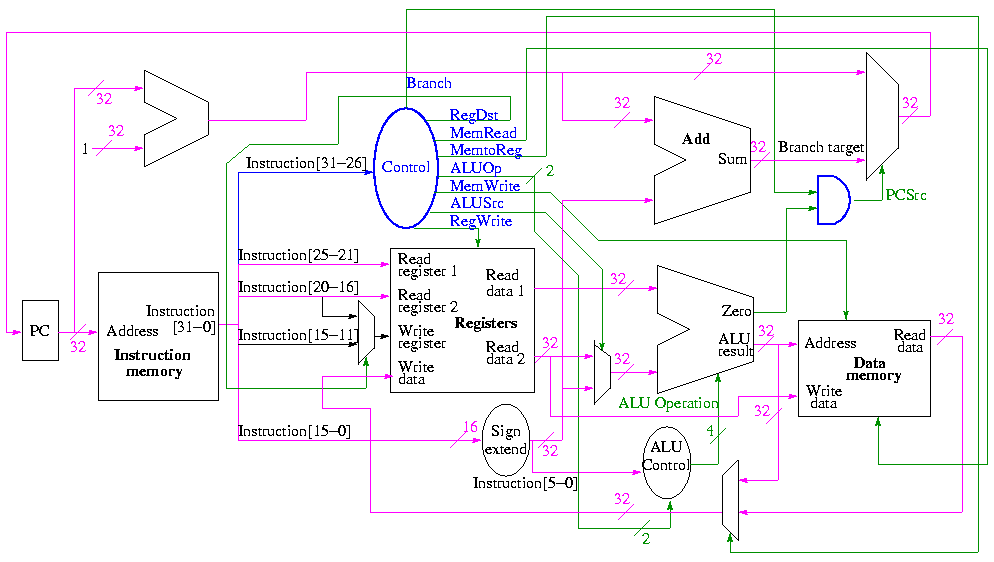
\includegraphics[width=\textwidth]{images/pipeline.png}


\section{MIPS Commands and Format}
\noindent
\begin{tabular}{p{1.25in}|p{.35in}|p{.35in}|p{.35in}|p{.35in}|p{.35in}|p{.35in}|}
  \cline{2-7}
  R-Format            & op & rs   & rt   & rd   & shamt & funct \\ \cline{2-7}
  Bits                & 6  & 5    & 5    & 5    & 5     & 6     \\ \cline{2-7}
  add \$r1,\$r2,\$r3  & 0  & \$r2 & \$r3 & \$r1 & 0     & 32    \\ \cline{2-7}
  addu \$r1,\$r2,\$r3 & 0  & \$r2 & \$r3 & \$r1 & 0     & 33    \\ \cline{2-7}
  sub \$r1,\$r2,\$r3  & 0  & \$r2 & \$r3 & \$r1 & 0     & 34    \\ \cline{2-7}
  subu \$r1,\$r2,\$r3 & 0  & \$r2 & \$r3 & \$r1 & 0     & 35    \\ \cline{2-7}
\end{tabular}

\vspace{.1in}\noindent
\begin{tabular}{p{1.25in}|p{.35in}|p{.35in}|p{.35in}|p{1.38in}|}
  \cline{2-5}
  I-Format             & op & rs   & rt   & address \\ \cline{2-5}
  Bits                 & 6  & 5    & 5    & 16      \\ \cline{2-5}
  lw \$r1,off(\$r2)    & 35 & \$r2 & \$r1 & off     \\ \cline{2-5}
  sw \$r1,off(\$r2)    & 43 & \$r2 & \$r1 & off     \\ \cline{2-5}
  beq \$r1,\$r2, label & 4  & \$r1 & \$r2 & label   \\ \cline{2-5}
\end{tabular}

\noindent
\begin{tabular}{llccc}
Mnemonic & Meaning                                  & Type & Opcode & Funct \\\hline
add	     & Add	                                    & R	   & 0x00   & 0x20 \\
addi     & Add Immediate	                        & I    & 0x08   & NA \\
addiu    & Add Unsigned Immediate	                & I    & 0x09   & NA \\
addu     & Add Unsigned	                            & R    & 0x00   & 0x21 \\
and      & Bitwise AND	                            & R    & 0x00   & 0x24 \\
andi     & Bitwise AND Immediate	                & I    & 0x0C   & NA \\
beq      & Branch if Equal	                        & I    & 0x04   & NA \\
bne      & Branch if Not Equal	                    & I    & 0x05   & NA \\
div      & Divide	                                & R    & 0x00   & 0x1A \\
divu     & Unsigned Divide	                        & R    & 0x00   & 0x1B \\
j        & Jump to Address	                        & J    & 0x02   & NA \\
jal      & Jump and Link     	                    & J    & 0x03   & NA \\
jr       & Jump to Address in Register	            & R    & 0x00   & 0x08 \\
lbu      & Load Byte Unsigned	                    & I    & 0x24   & NA \\
lhu      & Load Halfword Unsigned	                & I    & 0x25   & NA \\
lui      & Load Upper Immediate	                    & I    & 0x0F   & NA \\
lw       & Load Word	                            & I    & 0x23   & NA \\
mfhi     & Move from HI Register	                & R    & 0x00   & 0x10 \\
mflo     & Move from LO Register	                & R    & 0x00   & 0x12 \\
mfc0     & Move from Coprocessor 0 	                & R    & 0x10   & NA \\
mult     & Multiply	                                & R    & 0x00   & 0x18 \\
multu    & Unsigned Multiply     	                & R    & 0x00   & 0x19 \\
nor      & Bitwise NOR (NOT-OR)	                    & R    & 0x00   & 0x27 \\
xor      & Bitwise XOR (Exclusive-OR)	            & R    & 0x00   & 0x26 \\
or       & Bitwise OR	                            & R    & 0x00   & 0x25 \\
ori      & Bitwise OR Immediate	                    & I    & 0x0D   & NA \\
sb       & Store Byte	                            & I    & 0x28   & NA \\
sh       & Store Halfword	                        & I    & 0x29   & NA \\
slt      & Set to 1 if Less Than	                & R    & 0x00   & 0x2A \\
slti     & Set to 1 if Less Than Immediate	        & I    & 0x0A   & NA \\
sltiu    & Set to 1 if Less Than Unsigned Immediate	& I    & 0x0B   & NA \\
sltu     & Set to 1 if Less Than Unsigned	        & R    & 0x00   & 0x2B \\
sll      & Logical Shift Left	                    & R    & 0x00   & 0x00 \\
srl      & Logical Shift Right (0-extended)	        & R    & 0x00   & 0x02 \\
sra      & Arithmetic Shift Right (sign-extended)	& R    & 0x00   & 0x03 \\
sub      & Subtract	                                & R    & 0x00   & 0x22 \\
subu     & Unsigned Subtract	                    & R    & 0x00   & 0x23 \\
sw       & Store Word	                            & I    & 0x2B   & NA \\
\end{tabular}

\vspace{.1in}\noindent
\begin{tabular}{lcp{.2in}lc}\hline
Function          & ALU Control  && Function          & ALU Control  \\\hline
And               & 0000         && Subtract          & 0110         \\
Or                & 0001         && Set on Less Than  & 0111         \\
Add               & 0010         && Nor               & 1100         \\\hline
\end{tabular}

\vspace{.1in}\noindent
\begin{tabular}{|l|ccc|ccc|cc|}\hline
&\multicolumn{3}{|c|}{Ex Stage} &\multicolumn{3}{|c|}{Mem Stage} & \multicolumn{2}{|c|}{W/B Stage} \\\cline{2-9}
            & Reg & ALU & ALU &        & Mem  & Mem   & Reg   & Mem    \\
Instruction & Dst & Op  & Src & Branch & Read & Write & Write & to Reg \\\hline
lw          & 0   & 00  & 1   & 0      & 1    & 0     & 1     & 1      \\
sw          & x   & 00  & 1   & 0      & 0    & 1     & 0     & x      \\\hline
beq         & x   & 01  & 0   & 1      & 0    & 0     & 0     & x      \\
R-Type      & 1   & 10  & 0   & 0      & 0    & 0     & 1     & 0      \\\hline
\end{tabular}
